% !TEX root = ../BookTemplate.tex
%%%%%%%%%%%%%%%%%%%%%%%%%%%%%%%%%%%%%%%%%%%%%%%%%%%%%%%%%%%%%%%%%%%%%%%%%%%%%%%%%%
\chapter{คณิตศาสตร์สำหรับการวิเคราะห์เชิงปริมาณ}

ในบทแรก เราจะเริ่มจากการปูพื้นฐานคณิตศาสตร์ที่จำเป็นจะต้องใช้ในการเรียนรู้เนื้อหาวิชาการวิเคราะห์เชิงปริมาณกันก่อน
ทั้งนี้นักศึกษาไม่จำเป็นจะต้องศึกษาทั้งบทภายในครั้งเดียว เนื่องจากแต่ละบทนั้นจะมีคณิตศาสตร์ที่ต้องใช้แตกต่างกันไป นักศึกษาสามารถใช้บทนี้เป็นนบททบทวนก่อนขึ้นเนื้อหาหลักในแต่ละบทได้

สำหรับทางอาจารย์ผู้สอนนั้น ไม่ควรที่จะใช้บทนี้เป็นบทเรียนหลักที่สอนทั้งหมดภายในคราวเดียว เนื่องจากจนกว่าจะถึงตอนที่นักศึกษาจะต้องใช้จริงนั้น นักศึกษาเองก็อาจจะจำรายละเอียดไม่ได้แล้ว
ดังนั้น ทางผู้เขียนจึงขอแนะนำว่าให้หยิบไปบางส่วนขึ้นกับเนื้อหาหลักที่กำลังจะสอน และไม่ควรมีการออกสอบเก็บคะแนนสำหรับบทนี้ เนื่องจากเป็นความรู้พื้นฐานของเนื้อหาหลัก

อาจารย์ผู้สอนหรือนักศึกษาที่ศึกษาด้วยตัวเองสามารถใช้แผนภาพด้านล่างนี้เป็นแนวทางในการศึกษาในแต่ละหัวข้อ:

\begin{center}
\resizebox{\textwidth}{!}{\begin{tikzpicture}[
  font=\footnotesize,
  box/.style={rectangle, draw, text width=3.2cm, align=center, minimum height=1.2cm},
  arrow/.style={-{Stealth}, thick},
  node distance=1.2cm and 1.5cm
]

% กล่องเหตุผลเชิงปริมาณด้านล่าง
\node[box, fill=yellow!20] (reason) at (0,0) {เหตุผลเชิงปริมาณ};

% กลุ่มบทหลักแนวนอน
\node[box, fill=green!15, above=2.3cm of reason, xshift=-6.5cm] (ch2) {บทที่ 2\\โปรแกรมเชิงเส้น};
\node[box, fill=blue!10, right=1.5cm of ch2] (ch3) {บทที่ 3\\จำลองสถานการณ์};
\node[box, fill=blue!10, right=1.5cm of ch3] (ch4) {บทที่ 4\\การตัดสินใจ};
\node[box, fill=blue!10, right=1.5cm of ch4] (ch5) {บทที่ 5\\ทฤษฎีเกม};
\node[box, fill=blue!10, right=1.5cm of ch5] (ch6) {บทที่ 6\\ความน่าจะเป็น};
\node[box, fill=blue!10, right=1.5cm of ch6] (ch7) {บทที่ 7\\แถวคอย};

% คณิตศาสตร์พื้นฐานด้านล่างซ้าย
\node[box, below=1.5cm of ch2] (linear) {ระบบสมการ};
\node[box, below=1.5cm of ch5] (matrix) {เมทริกซ์};
\node[box, below=1.5cm of ch6] (prob) {ความน่าจะเป็น};

% ลูกศรจากคณิตศาสตร์พื้นฐาน
\draw[arrow] (linear.north) -- (ch2.south);
\draw[arrow] (matrix.north) -- (ch2.south);
\draw[arrow] (matrix.north) -- (ch5.south);
\draw[arrow] (prob.north) -- (ch3.south);
\draw[arrow] (prob.north) -- (ch4.south);
\draw[arrow] (prob.north) -- (ch6.south);
\draw[arrow] (prob.north) -- (ch7.south);

% ลูกศรจากเหตุผลเชิงปริมาณ
\foreach \x in {ch2, ch3, ch4, ch5, ch6, ch7}
  \draw[draw=red, dashed, -{Stealth}, thick] (reason.north) -- (\x.south);

\end{tikzpicture}}
\end{center}

\noindent จากแผนภาพจะเห็นว่าหัวข้อการให้เหตุผลเชิงปริมาณเป็นเนื้อหาสำคัญของบทนี้ที่จะข้ามไม่ได้ เนื่องจากเป็นบทที่ว่าด้วยทักษะการแปลปัญหาโลกจริงให้เป็นปัญหาทางคณิตศาสตร์ หรือกล่าวได้ว่าเป็นหัวข้อเกี่ยวกับ mathematical literacy ซึ่งจากประสบการณ์ของผู้เขียนนั้น พบว่านักเรียนนักศึกษาส่วนใหญ่ที่เรียนหัวข้อทางคณิตศาสตร์ หรือหัวข้อประยุกต์ทางคณิตศาสตร์ไม่เข้าใจ ไม่ได้เกิดจากการเรียนดนื้อหาในหัวข้อไม่เข้าใจ แต่เกิดจากการที่ไม่เข้าใจตั้งแต่แนวคิดตั้งต้นที่จะเชื่อมปัญหาในโลกจริงให้กลายเป็นปัญหาทางคณิตศาสตร์และใช้เครื่องมือทางคณิตศาสตร์เข้าไปช่วยแก้ปัญหา ซึ่งทางผู้เขียนค่อนข้างมีความเชื่อว่าสิ่งที่ยากไม่ใช่การเรียนเครื่องมือคณิตศาสตร์ เพราะอยากน้อยก็ใช้วิธีจำไปสอบ หรือตอนทำงานจริงก็เปิดคู่มือทำตามได้ แต่สิ่งที่ยากจริง ๆ คือการที่จะนำคณิตศาสตร์และปัญหาจริงมาเชื่อมโยงกันอย่างไร ดังนั้นจึงขอเน้นย้ำว่าหัวข้อการให้เหตุผลเชิงปริมาณนั้น ถึงแม้จะอยู่หัวข้อสุดท้ายของบท แต่ก็ไม่ควรละเลย

\newpage
\section{ระบบสมการเชิงเส้น}\label{section:linear}
ในบทที่ \ref{chapter:linprog} เราจะเรียนเกี่ยวกับการหาค่ามากสุดหรือน้อยสุด (เรียกว่าการทำ optimization) กับปัญหาที่ทั้งฟังก์ชันจุดประสงค์และเงื่อนไขอยู่ในรูปแบบที่เรียกว่า \textbf{รูปแบบเชิงเส้น} (linear form) กล่าวคือ เป็นรูปแบบที่ตัวแปรจะไม่มีการดำเนินการอื่นเลยนอกจากการบวกหรือลบ (ยกเว้นการคูณด้วยค่าคงที่ เพราะค่าคงที่ไม่ใช่ตัวแปร) ดังนั้นเราจะมาศึกษาเกี่ยวกับพื้นฐานของระบบเชิงเส้นเบื้องต้นกันในหัวข้อนี้ ซึ่งเราจะเริ่มด้วยการทำความเข้าใจสิ่งที่เรียกว่าเชิงเส้นกันในหัวข้อย่อย \ref{subsection:linear} และต่อด้วยระบบสมการเชิงเส้นในรูปแบบของความหมายเชิงเรขาคณิตรวมถึงการแก้สมการเบื้องต้นสำหรับผู้ที่ไม่มีพื้นฐานการแก้ระบบสมการฃ

ทั้งนี้ ก่อนที่จะเริ่มเนื้อหาจริง ๆ จะมี 2 คำสำคัญที่ต้องแยกความหมายให้ได้ นั่นคือ\textbf{ค่าคงที่} (constant) และ\textbf{ตัวแปร} (variable) โดยที่ค่าคงที่คือสิ่งที่ถูกกำหนดค่าตายตัวมาแล้วตั้งแต่แรก ถึงแม้ในการเขียนบางครั้งจะใช้ตัวอักษรภาษาอังกฤษก็ตาม แต่ตัวแปรคือสิ่งที่สามารถเปลี่ยนค่าได้ทำให้ระบบได้ผลลัพธ์ที่เปลี่ยนไป โดยถ้าเปรียบเทียบกับระบบการทำงานเครื่องจักรแปลสภาพวัตถุดิบ ค่าคงที่อาจเทียบได้กับรุ่นของอะไหล่ส่วนต่าง ๆ ซึ่งในบางครั้ง ถ้าเราเปลี่ยนค่าคงที่ไปก็คือเป็นการกล่าวถึงคนละระบบหรือคนละเครื่องจักรทันที แต่เมื่อเรามีเครื่องจักรแล้ว วัตถุดิบที่ใส่เข้าไปเปรียบเสมือนเป็นตัวแปรที่ในเครื่องจักรเครื่องนั้นจะให้ผลผลิตเป็นอะไรออกมาขึ้นกับว่าเราใส่วัตถุดิบหรือตัวแปรอะไรเข้า

ไม่ว่าจะค่าคงที่หรือตัวแปรก็ตาม ถ้าเราอธิบายคณิตศาสตร์ในเลเวลของการอธิบายเชิงนามธรรม ก็มักจะใช่ตัวอักษรภาษาอังกฤษทั้งคู่ ดังนั้นจงพึงละลึกไว้เสมอว่าตัวอักษรภาษาอังกฤษไม่ใช่ตัวแปรเสมอไป จะเป็นค่าคงที่หรือตัวแปร ขึ้นอยู่กับบริบทหรือหน้าที่ของสิ่งที่เรากำลังอธิบาย

\subsection{ฟังก์ชันเชิงเส้นและสมการเชิงเส้น} \label{subsection:linear}
ก่อนอื่น เราจะมาเริ่มกันที่นิยามของสิ่งต่าง ๆ ที่เกี่ยวข้องกับหัวข้อนี้กันก่อน
\begin{definition}{Linear Expression, Linear Equation and Linear Function}{}
    \textbf{นิพจน์เชิงเส้น} (Linear Expression) ของตัวแปร $x_1, \dots, x_n$ คือรูปแบบนิพจน์ทางคณิตศาสตร์ที่อยู่ในรูปแบบ $$c_0 + c_1x_1 + \cdots + c_nx_n$$ โดยที่ $c_i$ คือค่าคงที่ กล่าวคือไม่มี 2 ตัวแปรใด ๆ ที่ดำเนินการอื่นนอกจากการบวกหรือลบ ยกเว้นการคูณกันระหว่างค่าคงที่กับตัวแปร (ทั้งนี้เรายังคงจัดให้นิพจน์ที่มีแต่ค่าคงที่เป็นนิพจน์เชิงเส้นเช่นกัน)

    \textbf{สมการเชิงเส้น} (Linear Equation) คือสมการ (การเท่ากัน) ที่ทั้งสองฝั่งของสมการอยู่ในรูปแบบนิพจน์เชิงเส้น

    \textbf{ฟังก์ชันเชิงเส้น} (Linear Function) คือฟังก์ชันที่กำหนดกฏการคำนวณด้วยนิพจน์เชิงเส้น กล่าวคือ ฟังก์ชัน $f$ จะเป็นฟังก์ชันเชิงเส้นของตัวแปร $x_1, \dots, x_n$ ถ้า
    $$
    f(x_1, \dots, x_n) = c_0 + c_1x_1 + \cdots + c_nx_n
    $$
\end{definition}
สาเหตุที่เรียกว่าเชิงเส้น ก็มีที่มามาจากเส้นตรงในเรขาคณิต ซึ่งคือแนวทางการเดินทางที่มีพฤติกรรมว่าอัตราการเปลี่ยนค่ามีค่าคงที่และไม่ขึ้นกับค่าคงตัวแปรอื่น โดยจะได้นำตัวอย่างมาอธิบายในหัวข้อถัดไป
\newpage
\subsubsection{ตัวอย่างความสัมพันธ์เชิงเส้น 2 มิติ: กราฟเส้นตรง}
\paragraph{สมการสู่เส้นตรง}
ขอเริ่มจากสิ่งที่ง่ายกว่า ซึ่งคือเมื่อมีสมการแล้วอยากได้กราฟเส้นตรงของสมการ

\begin{enumerate}
    \item \textbf{กรณีไม่ได้ผ่านจุดกำเนิด}: สามารถทำได้โดยการหาจุดตัดแกน $x$ และจุดตัดแกน $y$
    \begin{center}
        \begin{tikzpicture}[scale=1.2, >=Stealth]
        
          % แกน
          \draw[->] (-0.5,0) -- (5,0) node[right] {$x$};
          \draw[->] (0,-0.5) -- (0,4) node[above] {$y$};
        
          % เส้นตรง
          \draw[thick, blue, <->] (-0.5,4) -- (3.5,-0.5);
        
          % จุด A และ B
          % \filldraw[black] (1,1) circle (1pt) node[below left] {$A$};
          % \filldraw[black] (3.5,2.5) circle (1pt) node[above right] {$B$};
        
        
          % สมการตรงกลางระหว่าง A กับ B
          \node at ($(3.5,0.25)$) {$(a,0)$};
          \node at ($(0.5,3.5)$) {$(0,b)$};
        
        \end{tikzpicture}
    \end{center}
    \begin{itemize}

        \item \textbf{จุดตัดแกน $x$} คือจุดที่มีค่า $y=0$ ซึ่งจะอยู่ในรูปแบบ $(a,0)$ และสามารถหาได้จากการแทนค่า $y=0$ ลงในสมการแล้วแก้สมการหาค่า $x$
        \item ในทำนองเดียวกัน เราก็สามารถหา\textbf{จุดตัดแกน $y$} ในรูป $(0,b)$ ได้ด้วยการแทนค่า $x=0$ แล้วแก้สมการหาค่า $y$
        
    \end{itemize}
    \begin{example}
        {วาดกราฟเส้นตรงที่ไม่ผ่านจุดกำเนิด}{}
        จงวาดกราฟของเส้นตรงของสมการ $3x + 4y = 24$
    \end{example}
    \newpage
    \item \textbf{กรณีผ่านจุดกำเนิด}: กรณีสมการอยู่ในรูป $Ax + By = 0$ ในกรณีนี้ทั้งระยะตัดแกน $x$ และระยะตัดแกน $y$ ต่างก็เป็น 0 ทั้งคู่ จึงทำให้จุดทั้ง 2 คือจุดเดียวกันคือจุด $(0,0)$ เพราะฉะนั้น จึงไม่มี 2 จุดให้ลากเชื่อมได้โดยง่ายเหมือนกรณีที่ผ่านมา
    \begin{center}
        \begin{tikzpicture}[scale=1.2, >=Stealth]
        
          % แกน
          \draw[->] (-0.5,0) -- (5,0) node[right] {$x$};
          \draw[->] (0,-0.5) -- (0,4) node[above] {$y$};
        
          % เส้นตรง
          \draw[thick, blue, <->] (-0.5,-0.35) -- (5,3.5);
        
          % จุด A และ B
          % \filldraw[black] (1,1) circle (1pt) node[below left] {$A$};
          % \filldraw[black] (3.5,2.5) circle (1pt) node[above right] {$B$};
        
        
          % สมการตรงกลางระหว่าง A กับ B
          \node at ($(0.5,-0.25)$) {$(0,0)$};
        
        \end{tikzpicture}
    \end{center}
    ในกรณีนี้เราสามารถแก้ปัญหาได้โดยการหาจุดที่อื่นที่ไม่จำเป็นต้องอยู่บนแกนก็ได้ เช่นอาจจะแทนค่า $x=1$ (หรือค่าอื่น ๆ แล้วแต่ความสะดวก) แล้วแก้สมการหาค่า $y$ ได้จุด $(1,y)$ แล้วลากเชื่อมกับจุด $(0,0)$
    \begin{example}
        {วาดกราฟเส้นตรงที่ผ่านจุดกำเนิด}{}
        จงวาดกราฟของเส้นตรงของสมการ $3x + 4y = 0$
    \end{example}
\end{enumerate}
\newpage
\paragraph{เส้นตรงสู่สมการ}
\begin{wrapfigure}{l}{0.5\textwidth}
 \centering~
  % \vspace{1ex}
    \begin{tikzpicture}[scale=1.2, >=Stealth]
    
      % แกน
      \draw[->] (-0.5,0) -- (5,0) node[right] {$x$};
      \draw[->] (0,-0.5) -- (0,4) node[above] {$y$};
    
      % เส้นตรง
      \draw[thick, blue, -{Stealth}] (1,1) -- (3.5,2.5);
    
      % จุด A และ B
      \filldraw[black] (1,1) circle (1pt) node[below left] {$A$};
      \filldraw[black] (3.5,2.5) circle (1pt) node[above right] {$B$};
    
      % เส้นประสามเหลี่ยมมุมฉาก
      \draw[dashed] (1,1) -- (3.5,1) node[midway, below] {$\Delta x$};
      \draw[dashed] (3.5,1) -- (3.5,2.5) node[midway, right] {$\Delta y$};
    
      % สมการตรงกลางระหว่าง A กับ B
      \node at ($(0,2)!0.5!(3.5,2.5) + (0,0.3)$) {$\displaystyle \frac{\Delta y}{\Delta x} = \text{ค่าคงที่}$};
    
    \end{tikzpicture}
    ~\vspace{4ex}
\end{wrapfigure}%
ซึ่งเมื่อลองกำหนดให้มีจุดตั้งต้น $A(x_0, y_0)$ เป็นจุดคงที่และสมมติว่า $B(x,y)$ คือจุดตัวแปรใด ๆ ที่อยู่ในแนวเส้นตรงนั้น และสมมติว่าอัตราคงที่ดังกล่าวคือ $m$ จะได้สมการว่า
$$
\frac{y-y_0}{x-x_0} = m
$$
และท้ายที่สุด จะได้สมการออกมาในรูปแบบ
$
y = (y_0 - kx_0) + mx
$
ซึ่งจะเห็นว่ารูปสมการที่ได้จะอยู่ในรูปแบบเชิงเส้น โดยที่มี $c_0 = y_0 - kx_0$ เป็นพจน์ค่าคงที่ และถ้าพิจารณาในรูปแบบของเส้นตรงทางเรขาคณิต ค่า $m$ ที่เป็นค่าคงที่ที่คูณอยู่หน้าตัวแปร $x$ จะเรียกว่า \textbf{ความชัน} (slope)

\begin{example}{การหาสมการของเส้นตรง $(x,y)$}{}
    จงหาสมการของเส้นตรงที่ผ่านจุด (3,2) และมีความชันเท่ากับ 3
\end{example}
\begin{tikzpicture}[scale=0.9, >=Stealth]

  % แกน
  \draw[->] (0,0) -- (7,0) node[right] {$x$};
  \draw[->] (0,0) -- (0,7) node[above] {$y$};

  % จุดเริ่มต้น A = (3,2)
  \coordinate (A) at (3,2);
  \node[below left] at (A) {$(3,2)$};
  \filldraw (A) circle (2pt);

  % คำนวณจุด B เฉย ๆ เพื่อใช้เส้น ไม่แสดงในภาพ
  \coordinate (B) at ($(A)+(1,3)$);

  % เส้นตรงผ่าน A ที่ชัน = 3
  \draw[blue, thick, -{Stealth}] (2.5,0.5) -- (4.5,6.5);

  % วาดสามเหลี่ยมมุมฉากเส้นประ
  \draw[dashed] (A) -- ($(A)+(1,0)$) node[midway, below] {$\Delta x$};
  \draw[dashed] ($(A)+(1,0)$) -- (B) node[midway, right] {$\Delta y$};

  % สมการความชัน
  \node at ($(A)!0.5!(B) + (0,0.5)$)
    {$\displaystyle \frac{\Delta y}{\Delta x} = 3$};
\end{tikzpicture}

\newpage
\begin{example}{การหาสมการของเส้นตรง $(x,y)$}{}
    จงหาสมการของเส้นตรงที่ผ่านจุด (4,-1) และจุด (-1,2)
\end{example}
\begin{tikzpicture}[scale=0.8, >=Stealth]

  % แกน
  \draw[->] (-2,0) -- (6,0) node[right] {$x$};
  \draw[->] (0,-2) -- (0,4) node[above] {$y$};

  % จุด A = (4, -1), B = (-1, 2)
  \coordinate (A) at (4,-1);
  \coordinate (B) at (-1,2);

  % เส้นตรงผ่าน A และ B
  \draw[thick, blue, -{Stealth}] (4,-1) -- (-1,2);

  % วงกลมจุด A, B
  \filldraw[black] (A) circle (2pt) node[below right] {$(4,\,-1)$};
  \filldraw[black] (B) circle (2pt) node[above left] {$(\,-1,\,2)$};

\end{tikzpicture}

\newpage
\subsubsection{ตัวอย่างความสัมพันธ์เชิงเส้น 3 มิติ: กราฟระนาบ $x,y,z$}\label{subsubsection:plane}
เส้นตรงและสมการเส้นตรงที่ได้ศึกษาไปในหัวข้อที่แล้วนั้นเป็นตัวอย่างอย่างง่ายในระนาบพิกัด 2 มิติ (และตัวเส้นตรงเองเป็นวัตถุ 1 มิติ) กล่าวคือเรากำลังศึกษาวัตถุ 1 มิติในมุมมอง 2 มิติ
ในหัวข้อย่อยนี้เราจะศึกษาของที่มิติสูงขึ้นอีกขั้นหนึ่งในมุมมอง 3 มิติ (พิกัด $x,y,z$) โดยวัตถุเชิงเส้นในระบบ 3 มิติดังกล่าวสามารถเขียนได้อยู่ในรูป
$$
0 = Ax + By + Cz + K
$$
(เส้นตรงใน 2 มิติก็สามารถเขียนได้ในทำนองเดียวกันคือ $0 = Ax + By + K$) หรือเขียนในรูปแบบฟังก์ชันของค่า $z$ คือ
$$
z = ax + by + k
$$

% สำหรับนักศึกษาที่ไม่เคยเรียนวิชาแคลคูลัสหลายตัวแปรมาก่อนอาจจะยังไม่เคยรู้จักกราฟของสมการดังกล่าว ทว่าไม่ใช่เรื่องยากที่จะสามารถหากราฟของสมการดังกล่าว เพียงแค่เราใช้คุณสมบัติของความเป็นเชิงเส้นเข้ามาช่วยดังนี้

\begin{property}{เชิงเส้นในเชิงเส้น: กรณีตัวอย่าง 3 ตัวแปร}{}
    กำหนดความสัมพันธ์เชิงเส้น 3 ตัวแปร $$z = f(x,y) = ax + by + k$$
    ถ้าสมมติให้ตัวแปรตัวหนึ่งเป็นค่าคงที่ (สมมติว่าเป็น $x = x_0$) จะได้สมการที่เหลือ 2 ตัวแปรเป็น $$z = by + (ax_0 + k)$$
    กล่าวคือ เราจะได้สมการเส้นตรงของตัวแปร $y, z$ ซึ่งจะพบว่าไม่ว่าเราจะกำหนดตัวแปร $x$ ให้เป็นค่าคงที่ใด ๆ ก็ตาม เราจะยังคงได้เส้นตรงความชัน $b$ เท่าเดิม เปลี่ยนแค่พจน์ในวงเล็บซึ่งคือจุดตัดระนาบ $x-z$ (แนว $y = 0$) ซึ่งจะมีแนวทางเดินรอยตัดคือ $z = ax + k$
   
\end{property}


\def\a{-1}    % slope a
\def\b{2}
\def\k{8}      % intercept k
ตัวอย่างเช่นเราอยากวาดกราฟของสมการ $z = \a x + \b y + \k$\\

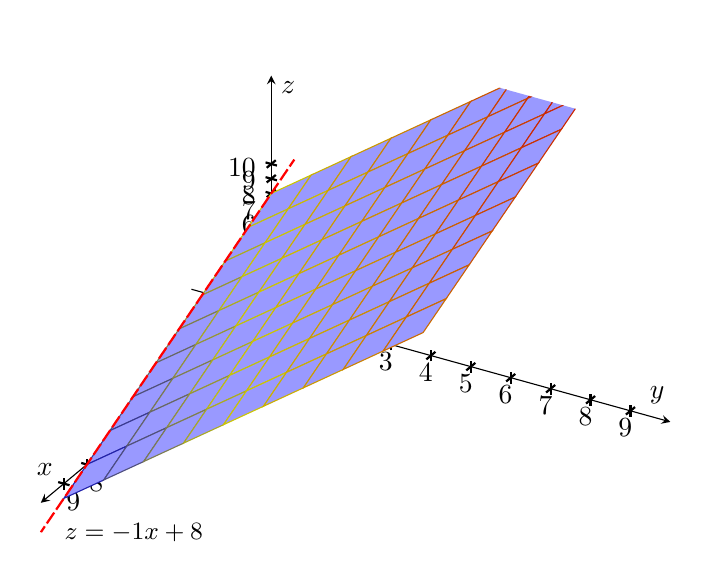
\begin{tikzpicture}
  \begin{axis}[
    view={120}{45},         % มุมกล้อง
    axis lines=center,
    xlabel={$x$}, ylabel={$y$}, zlabel={$z$},
    xmin=-2, xmax=10,
    ymin=-2, ymax=10,
    zmin=-2, zmax=16,
    xtick={1,2,3,4,5,6,7,8,9},
    ytick={1,2,3,4,5,6,7,8,9},
    ztick={0,1,...,10},
    xtick distance=1,
    ytick distance=1,
    ztick distance=1,
    tick style={black, thick},
    enlargelimits=false,
    grid=major,
    grid style={dotted},
    scale = 1.4
  ]

  \addplot3[
        surf,
      domain=0:9,
      color=blue!40!white,
      samples=10,
    ]
    ({x}, {y}, {\a*x + \b*y + \k});

   \addplot3[
    domain=-1:10,
    samples=2,
    dashed,
    thick,
    color=red
  ]
  ({x}, {0}, {\a*x + \k});  % x, y=0, z = ax + k

  \node at (axis cs:9,1.75, \a*10 + \k + 0) {\small $z = \a x + \k$};
  \end{axis}
\end{tikzpicture}

หลังจากที่ได้ลองพิจารณากราฟของสมการเชิงเส้น 3 ตัวแปรด้วยวิธีการกำหนดให้ตัวแปรหนึ่งเป็นค่าคงที่แล้วลองวาดเส้นตรงของสมการเชิงเส้น 2 ตัวแปรที่เหลือ
จะพบว่ารูปที่ได้ เปรียบเสมือนการเลื่อนเส้นตรงไปตามแนวของเส้นตรงเส้นอีกเส้นหนึ่ง ทำให้ได้ออกมาในลักษณะแผ่นเรียบที่เรียกว่า ``ระนาบ'' (plane)
ซึ่งคือวัตถุเชิงเส้นในระบบพิกัดฉาก 3 มิติ (ถึงแม้จะไม่ได้มีรูปร่างเป็นเส้นตรงก็ตาม)

\begin{example}{การหาสมการของเส้นตรง $(x,y)$}{}
    จงวาดกราฟของสมการระนาบ $3x + 5y - z = 5$\\
    (challenge: ถ้าต้องการเดินไต่ตามระนาบ เสมือนว่าระนาบคือส่วนหนึ่งของภูเขา จงหาว่าต้องหันหัวไปทางทิศไหนถึงจะขึ้นได้เร็วที่สุด -- ปัญหานี้จะเกี่ยวข้องกับหัวข้อการโปรแกรมเชิงเส้นที่อยู่ในบทที่ \ref{chapter:linprog})
\end{example}
\begin{tikzpicture}
  \begin{axis}[
    view={120}{45},         % มุมกล้อง
    axis lines=center,
    xlabel={$x$}, ylabel={$y$}, zlabel={$z$},
    xmin=-8, xmax=11,
    ymin=-8, ymax=11,
    zmin=-8, zmax=11,
    xtick={-7,-6,...,10},
    ytick={-7,-6,...,10},
    ztick={-7,-6,...,10},
    xtick distance=1,
    ytick distance=1,
    ztick distance=1,
    tick style={black, thick},
    enlargelimits=false,
    grid=major,
    grid style={dotted},
    scale = 3.5
  ]

  \end{axis}
\end{tikzpicture}
\newpage

\subsection{ระบบสมการเชิงเส้น: ความหมายเชิงรูปภาพของการแก้สมการ}
เมื่อพูดถึงสมการเชิงเส้นเพียงหนึ่งสมการ ผลเฉลยก็คือสิ่งที่แทนค่าตัวแปรเข้าไปแล้วเป็นจริง ตัวอย่างเช่นเรามีสมการเชิงเส้น 2 ตัวแปร $y = 3x + 5$ ก็จะได้ว่า $(0,5), (-2,-1)$ หรือ $(5,20)$ ต่างก็เป็นผลเฉลยของสมการดังกล่าว และยังมีอีกมากมายหลายจุดที่ต่างก็เป็นผลเฉลยของสมการนั้น
ซึ่งถ้ามองในรูปแบบการวาดกราฟ ผลเฉลยก็คือจุดในพิกัดฉากที่กราฟของสมการนั้นลากผ่านนั่นเอง

และเมื่อเรามีสมการเชิงเส้นมากกว่า 1 สมการมาพิจารณาพร้อมกัน สิ่งนั้นจะถูกเรียกว่า ``\textbf{ระบบสมการเชิงเส้น}" หรือก็คือระบบที่มีสมการเชิงเส้นหลายสมการ และผลเฉลยของระบบสมการเชิงเส้นก็คือจุดที่สอดคล้องทุกสมการในระบบ หรือก็คือเมื่อวาดรูปแล้ว ทุกกราฟจะลากผ่านจุดนั้นหรือก็คือ จุดตัดร่วมของทุกกราฟนั่นเอง

\subsubsection{ตัวอย่างระบบสมการเชิงเส้น 2 ตัวแปร: เส้นตรงตัดกัน}
เส้นตรง 2 เส้นที่แตกต่างในระบบพิกัดฉาก 2 มิติสามารถวางตัวกันได้ 2 แบบคือ (1) ตัดกัน 1 จุด และ (2) ขนานกัน
\begin{figure}[ht]
\centering

% === Axis ซ้าย: เส้นตัดกัน
\begin{minipage}[t]{0.45\textwidth}
\centering
\begin{tikzpicture}
\begin{axis}[
  axis lines=middle,
  xmin=-2, xmax=4,
  ymin=-2, ymax=4,
  xtick=\empty, ytick=\empty,
  xlabel={$x$}, ylabel={$y$},
  title={ตัดกัน 1 จุด},
  title style={font=\small}
]
\addplot[red, thick, domain=-1.5:3.5] {x + 1};
\addplot[blue, thick, domain=-1.5:3.5] {-0.5*x + 2};
\end{axis}
\end{tikzpicture}
\end{minipage}
\hfill
% === Axis ขวา: เส้นขนานกัน
\begin{minipage}[t]{0.45\textwidth}
\centering
\begin{tikzpicture}
\begin{axis}[
  axis lines=middle,
  xmin=-2, xmax=4,
  ymin=-2, ymax=4,
  xtick=\empty, ytick=\empty,
  xlabel={$x$}, ylabel={$y$},
  title={ขนานกัน},
  title style={font=\small}
]
\addplot[red, thick, domain=-1.5:3.5] {0.5*x + 1};
\addplot[blue, thick, domain=-1.5:3.5] {0.5*x - 1};
\end{axis}
\end{tikzpicture}
\end{minipage}

\caption{เส้นตรง 2 เส้นสามารถวางตัวได้ 2 แบบ: ตัดกัน (ซ้าย) และขนานกัน (ขวา)}
\label{fig:line-relations}
\end{figure}

คำถามสำคัญที่ตามมาจะมีดังนี้
\begin{enumerate}
    \item จะรู้ได้อย่างไรว่าสมการของเส้นตรง 2 เส้นนั้นเป็นเส้นที่แตกต่างกัน
    \item และเมื่อทราบว่าแตกต่างกันแล้วนั้น จะรู้ได้อย่างไรว่าขนานหรือตัดกัน
    \item และสุดท้าย เมื่อทราบแล้วว่าตัดกัน 1 จุด จะหาผลเฉลยดังกล่าวได้อย่างไร
\end{enumerate}

สำหรับคำถามที่ 1 นั้น ต้องพึงระวังไว้เสมอว่าถึงแม้สมการเชิงเส้น 2 สมการจะใช้สัมประสิทธิ์ไม่เหมือนกันก็อาจจะเป็นเส้นตรงเส้นเดียวกันได้ ตัวอย่างเช่น
\begin{align*}
    0 &= 3x + 5y - 7\\
    0 &= 15x + 25y - 35
\end{align*}
สมการทั้งสองนี้มีกราฟเส้นตรงรูปเดียวกัน (ทำไม?)

ในขณะที่ระบบสมการนี้
\begin{align*}
    0 &= 3x + 5y - 7\\
    0 &= 15x + 25y - 3
\end{align*}
เป็นกราฟเส้นตรง 2 เส้นที่ขนานกัน

\begin{example}{การแก้ระบบสมการ 2 ตัวแปร}{}
    จงแก้ระบบสมการ
    \begin{align*}
        0 &= 3x + 5y - 7\\
        0 &= -2x + 3y - 3
    \end{align*}
    พร้อมทั้งวาดรูปประกอบ
\end{example}
\newpage
\subsubsection{ตัวอย่างระบบสมการเชิงเส้น 3 ตัวแปร: ระนาบตัดกัน}
คำถามแรกที่ค่อนข้างง่ายคือ ``ถ้าระนาบ 2 แผ่นตัดกัน จะได้รอยตัดรูปอะไร?'' ทว่าการหาผลเฉลยของรอยตัดดังกล่าวกลับเป็นเรื่องยาก
และคำถามในทำนองเดียวกันคือ ``ถ้าเรามีระนาบ 2 แผ่น จะรู้ได้อย่างไรว่าระนาบตัดหรือไม่ตัดกัน''
~\vspace{5cm}

จากรูปแบบการตัดแบบต่าง ๆ จะพบว่าการที่จะได้ผลเฉลยแบบออกมา 1 จุดนั้น ต้องอาศัยระนาบตัดกัน 3 แผ่นเพื่อให้ได้จุดตัดร่วมออกมาเป็น 1 จุด
\begin{example}{การแก้ระบบสมการ 3 ตัวแปร}{}
    จงแก้ระบบสมการ
    \begin{align*}
        0 &= 3x + 5y - 9z - 7\\
        0 &= -2x + 3y + 2z - 3\\
        0 &= x + 6y + 3z +5
    \end{align*}
\end{example}
\newpage
\subsection{อสมการเชิงเส้น และการวาดกราฟของอสมการเชิงเส้น}


\section{การดำเนินการบนเมทริกซ์}
\subsection{เมทริกซ์}
\subsection{การคูณเมทริกซ์}
\subsection{การใช้เมทริกซ์สำหรับทฤษฎีกราฟเบื้องต้น}

\section{ความน่าจะเป็นเบื้องต้น}
\subsection{แนวคิดตั้งต้นสำหรับความน่าจะเป็น}
\subsection{ตัวแปรสุ่ม ค่าคาดหวัง ความอิสระ}
\subsection{กฏของเบย์}
\subsection{การแจกแจงความน่าจะเป็น}

\section{พื้นฐานการให้เหตุผลเชิงปริมาณ}\label{section:mathexpression}
\subsection{ทักษะการแปรคำพูดเป็นนิพจน์ทางคณิตศาสตร์}
\subsection{การเข้าใจจุดประสงค์และเงื่อนไขของปัญหา}